\openany\raggedright

\blankpage
\part[A mulher que virou tatu]{A mulher que\\ virou tatu}

\chapter*{}

\mbox{}\vspace*{\fill}

% \begin{verse}
% \letra{Q}{uando} a família se reunia, só se comia\\
% batata doce. Faziam roçado e plantavam\\
% batata doce. Só davam batata doce bichada\\
% para a velha comer. É o que davam à velha.\\
% Ela vivia com a família.
% \end{verse}

\begingroup\setlength{\linewidth}{.6\linewidth}

\letra{Q}{uando} a família se reunia, só se comia
batata doce. Faziam roçado e plantavam
batata doce. Só davam batata doce bichada
para a velha comer. É o que davam à velha.
Ela vivia com a família.

\vspace{2em}

% \begin{verse}
% \textit{Kadi besti pikin, itxa wani kiaki.\\
% Bai wakin hawen ni katsidan, kadi banaaki.\\
% Xena besti pimiski hawen pitimaken.\\
% Yuxabudan eskani kiaki.Hawen\\
% nabube hiwea.}
% \end{verse}

\letra{K}{adi} besti pikin, itxa wani kiaki.
Bai wakin hawen ni katsidan, kadi banaaki.
Xena besti pimiski hawen pitimaken.
Yuxabudan eskani kiaki.Hawen
nabube hiwea.

\vspace*{\fill}

\pagebreak
\thispagestyle{empty}
\begin{figure}
\vspace*{-.5cm}
\hspace*{-2.3cm}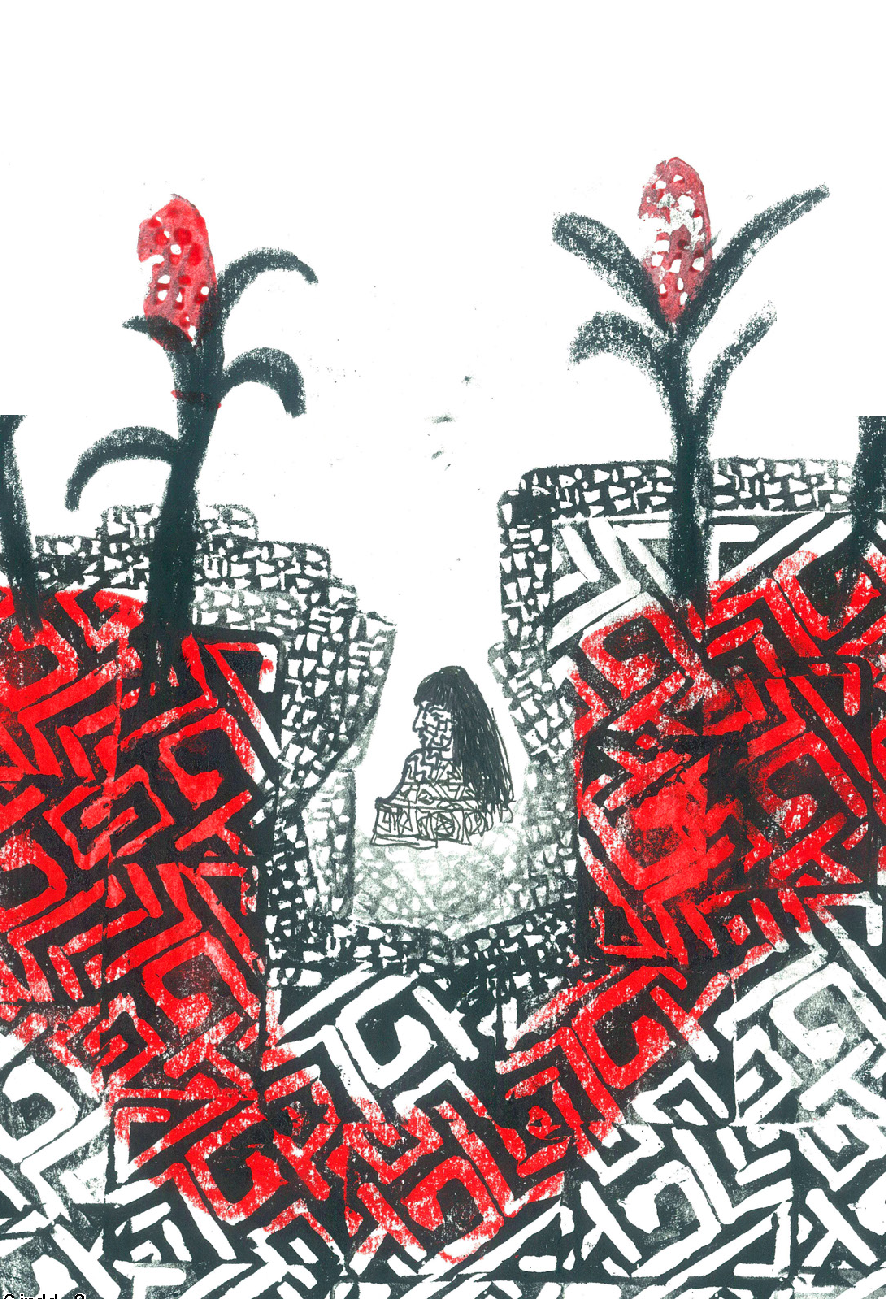
\includegraphics[width=140mm]{./imgs/img1.pdf}
\end{figure}

\chapter*{}

\mbox{}\vspace*{\fill}

% \begin{verse}
% A família dela fazia roçado e tinha\\
% um milharal. A velha desdentada\\
% não podia comer milho seco.
% \end{verse}

% \begin{verse}
% \textit{Hawen nabu bai waxun, xeki\\
% banaimabu. Yuxabudan xeta uma,\\
% haska waxun piti, kuxi pitima.}
% \end{verse}


\letra{A}{família} dela fazia roçado e tinha
um milharal. A velha desdentada
não podia comer milho seco.

\vspace{2em}

\letra{H}{awen} nabu bai waxun, xeki
banaimabu. Yuxabudan xeta uma,
haska waxun piti, kuxi pitima.

\vspace*{\fill}

\pagebreak
\thispagestyle{empty}
\begin{figure}
\vspace*{-.5cm}
\hspace*{-2.2cm}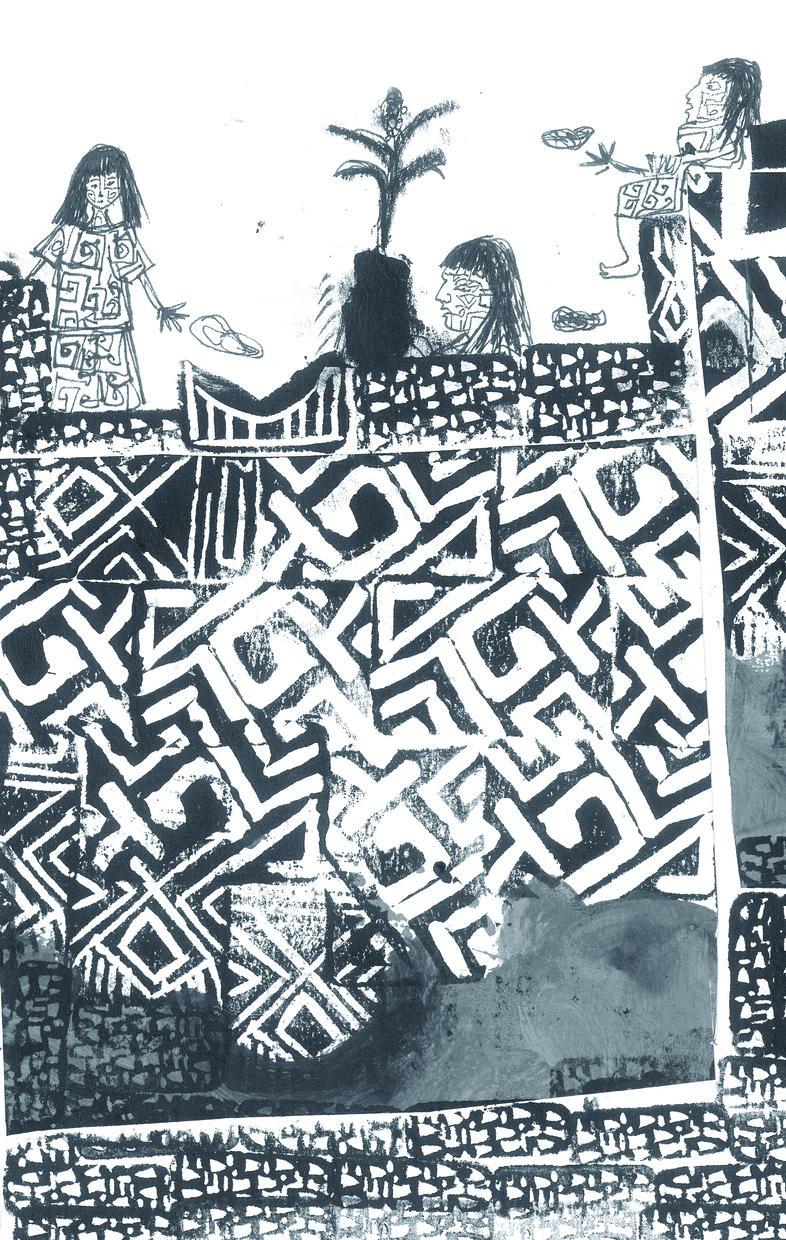
\includegraphics[width=138mm]{./imgs/img2.pdf}
\end{figure}

\chapter*{}

%\mbox{}\vspace*{\fill}
\vspace*{-\baselineskip}

% \begin{verse}
% Quando a velha vivia com\\
% a família, desperdiçava-se\\
% muito milho verde.\\
% Ela queria virar tatu, pois\\
% não podia comer o milho verde,\\
% visto que a família lhe dizia:\\
% --- Ô, velha, você só fica\\
% comendo o nosso milho verde.\\
% Ela respondia:\\
% --- Como só milho verde, por\\
% não poder comer milho seco.\\
% Não tenho dente.\\
% A mulher respondeu isso\\
% e ficou pensando no que\\
% a família lhe disse.
% \end{verse}

% \begin{verse}
% \textit{Hawen nabube hiwea,\\
% mawa xeki pati txakaaya.\\
% Yuxabudan yaix katsidan\\
% eskani kiaki. Haska waxun,\\
% pitima, xeki patxi besti piaya,\\
% hawen nabun itxaa:\\
% --- Yuxabun, min en xeki\\
% patxi besti piai, aka.\\
% Yuxabu yuikin:\\
% --- En haska waxun piti kuxi\\
% pitima. En xeta uma, en xeta\\
% umabin. Ainbun yuia, ainbu\\
% ninkaxun.}
% \end{verse}

\letra{Q}{uando} a velha vivia com
a família, desperdiçava-se
muito milho verde.
Ela queria virar tatu, pois
não podia comer o milho verde,
visto que a família lhe dizia:\break
--- Ô, velha, você só fica
comendo o nosso milho verde.
Ela respondia:\break
--- Como só milho verde, por
não poder comer milho seco.
Não tenho dente.\break
A mulher respondeu isso
e ficou pensando no que
a família lhe disse.

\vspace{2em}

\letra{H}{awen} nabube hiwea,
mawa xeki pati txakaaya.
Yuxabudan yaix katsidan
eskani kiaki. Haska waxun,
pitima, xeki patxi besti piaya,
hawen nabun itxaa:\break
--- Yuxabun, min en xeki
patxi besti piai, aka.
Yuxabu yuikin:\break
--- En haska waxun piti kuxi
pitima. En xeta uma, en xeta
umabin.\break
Ainbun yuia, ainbu
ninkaxun.

\vspace*{\fill}

\pagebreak
\thispagestyle{empty}
\begin{figure}
\vspace*{-.9cm}
\hspace*{-2.5cm}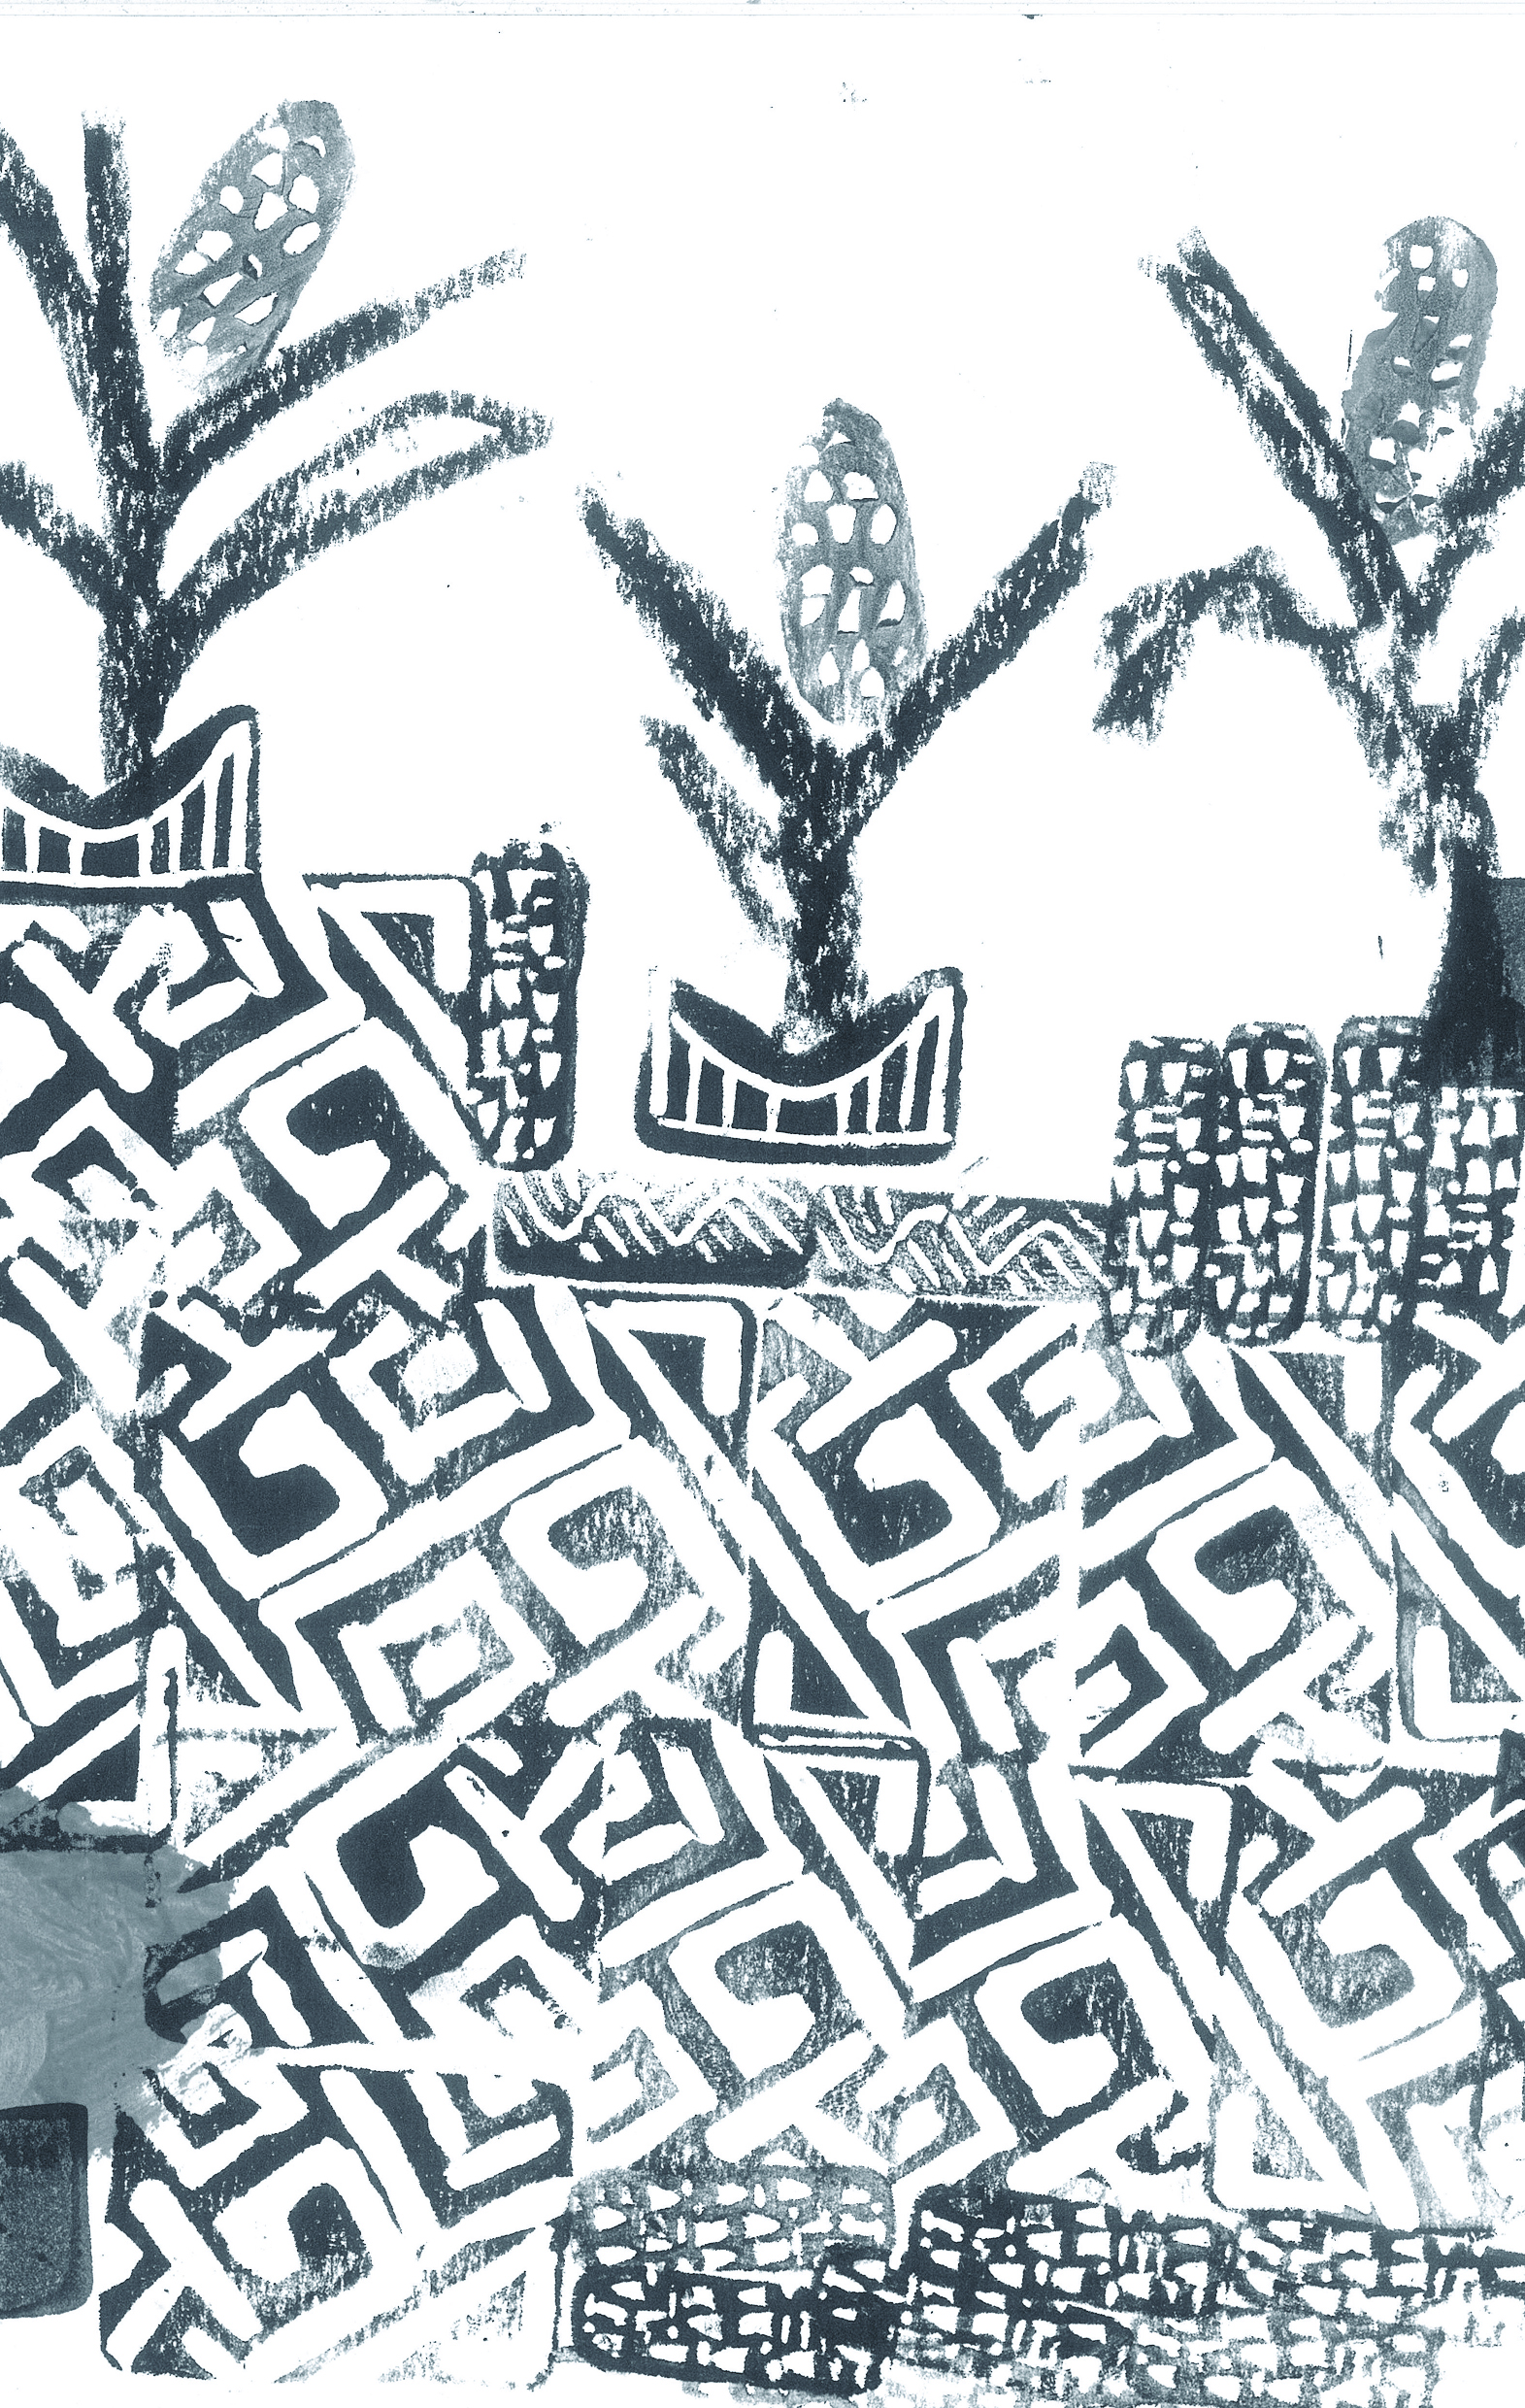
\includegraphics[width=143mm]{./imgs/img3.pdf}
\end{figure}

\chapter*{}

\vspace*{-\baselineskip}
%\mbox{}\vspace*{\fill}

% \begin{verse}
% Então ela foi sozinha mata\\
% adentro e, ao voltar, à\\
% tardezinha, disse à sua filha:\\
% --- Filha, eu vou virar tatu. Sou\\
% desdentada e por isso não posso\\
% comer milho verde. Vou embora.\\
% A filha respondeu-lhe:\\
% --- Mamãe, é por isso que\\
% você não pode comer?\\
% --- Minha filha, é. É por isso que\\
% não posso comer — respondeu-lhe.\\
% A filha replicou:\\
% --- Mamãe, então coma\\
% só milho verde!
% \end{verse}

% \begin{verse}
% \textit{Hanunkain, yuxabu ni medan\\
% ha mesti kaa, badi kaaya\\
% huxun, hawen bake yuia:\\
% --- En bake, eadan en yaixi kaai. En\\
% xeta uma. Haska waxun,\\
% piti kuxi pitima, en ikai, aka.\\
% Hawen bake yuikin:\\
% --- En ewan, min haska waxun\\
% pitimamen, aka. En bake, en haska\\
% waxun, pitimabin, aka.\\
% Hawen bake yuia:\\
% --- Ewan, xeki patxi\\
% besti piwe, aka.}
% \end{verse}

\letra{E}{ntão} ela foi sozinha mata
adentro e, ao voltar, à
tardezinha, disse à sua filha:\break
--- Filha, eu vou virar tatu. Sou
desdentada e por isso não posso
comer milho verde. Vou embora.
A filha respondeu-lhe:\break
--- Mamãe, é por isso que
você não pode comer?\break
--- Minha filha, é. É por isso que
não posso comer, respondeu-lhe.
A filha replicou:\break
--- Mamãe, então coma
só milho verde!

\vspace{2em}

\letra{H}{anunkain}, yuxabu ni medan
ha mesti kaa, badi kaaya
huxun, hawen bake yuia:\break
--- En bake, eadan en yaixi kaai. En
xeta uma. Haska waxun,
piti kuxi pitima, en ikai, aka.
Hawen bake yuikin:\break
--- En ewan, min haska waxun
pitimamen, aka. En bake, en haska
waxun, pitimabin, aka.
Hawen bake yuia:\break
--- Ewan, xeki patxi
besti piwe, aka.

\vspace*{\fill}

\pagebreak
\thispagestyle{empty}
\begin{figure}
\vspace*{-.5cm}
\hspace*{-2.2cm}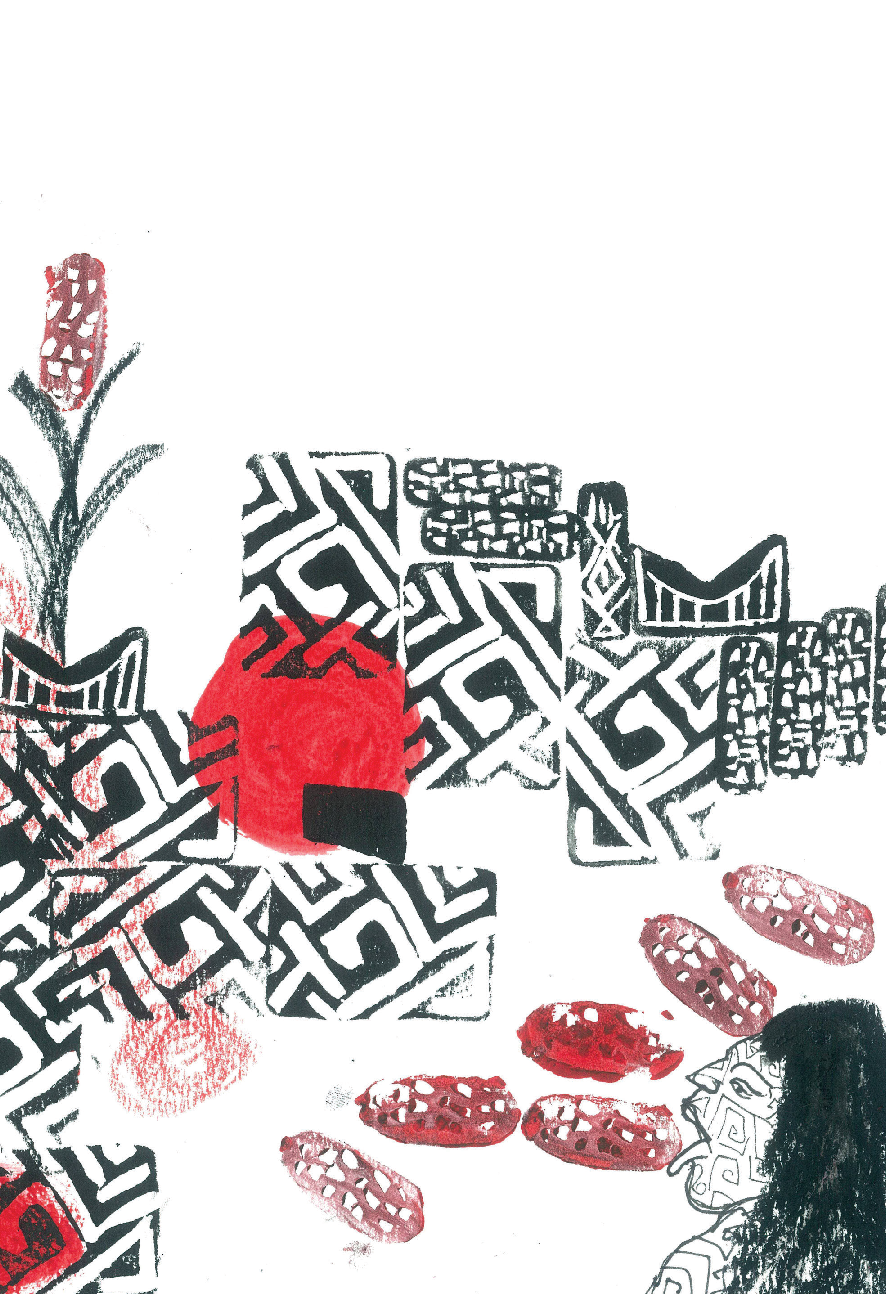
\includegraphics[width=138mm]{./imgs/img4.pdf}
\end{figure}

\chapter*{}

\mbox{}\vspace*{\fill}

% \begin{verse}
% A velha só comia milho\\
% verde por não poder comer\\
% milho seco, que é duro.\\
% Quando acabou o milho verde\\
% do roçado deles, os homens\\
% estavam zangados\\
% e lhe disseram:\\
% --- Velha, você acabou com o\\
% nosso roçado de milho verde.\\
% \end{verse}

% \begin{verse}
% \textit{Yuxabun xeki patxi besti piaya.\\
% Haska waxun, piti kuxi pitima.\\
% Hatun bai xeki patxi keyun waaya,\\
% hunibun sinaxun, yuxabu yuikin:\\
% --- Yuxabun, min en xeki\\
% patxi bai keyuna, aka.\\}
% \end{verse}

\letra{A}{velha} só comia milho
verde por não poder comer
milho seco, que é duro.
Quando acabou o milho verde
do roçado deles, os homens
estavam zangados
e lhe disseram:\break
--- Velha, você acabou com o
nosso roçado de milho verde.

\vspace{2em}

\letra{Y}{uxabun} xeki patxi besti piaya.
Haska waxun, piti kuxi pitima.
Hatun bai xeki patxi keyun waaya,
hunibun sinaxun, yuxabu yuikin:\break
--- Yuxabun, min en xeki
patxi bai keyuna, aka.

\vspace*{\fill}

\pagebreak
\thispagestyle{empty}
\begin{figure}
\vspace*{-1.3cm}
\hspace*{-2.5cm}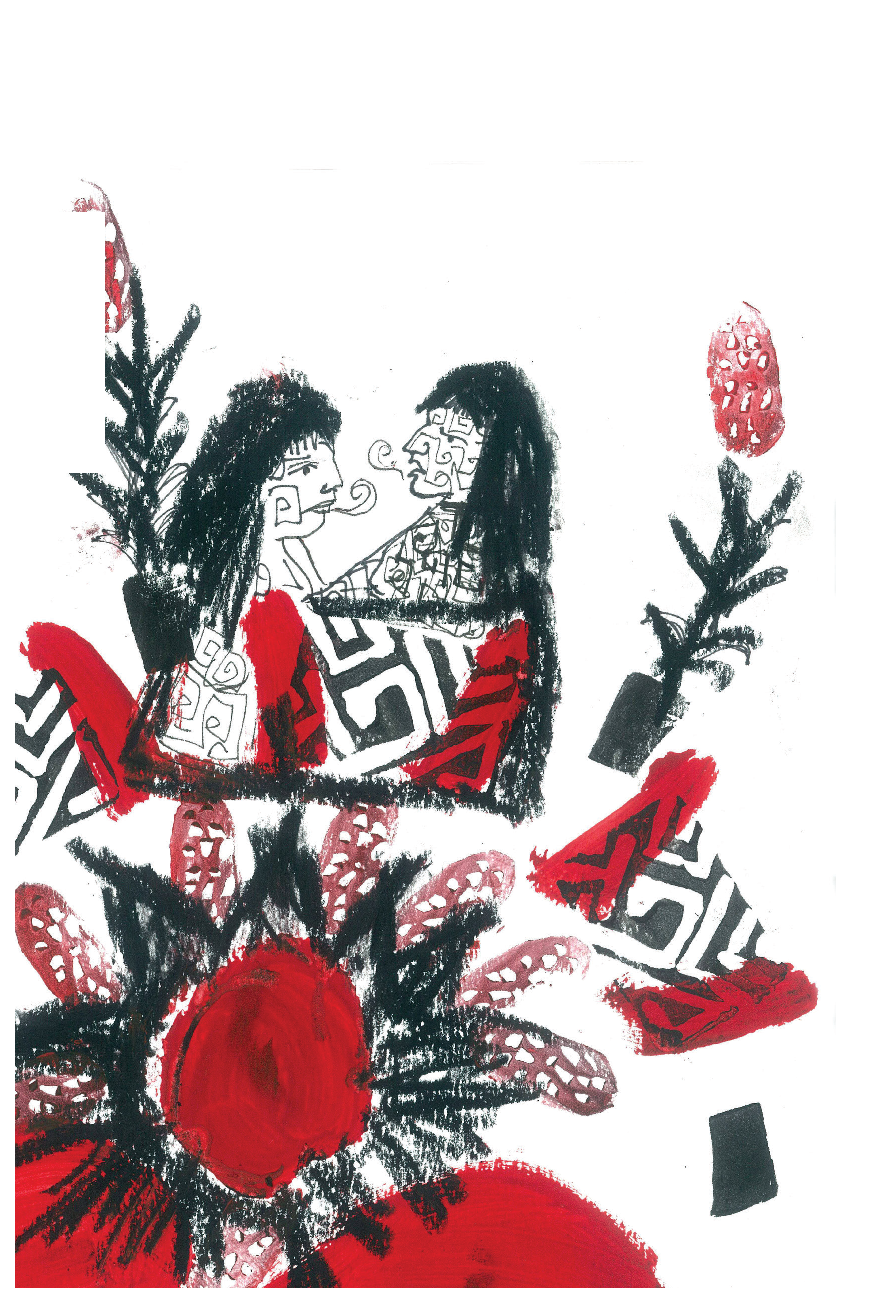
\includegraphics[width=145mm]{./imgs/img5.pdf}
\end{figure}

\chapter*{}

% \begin{verse}
% Ela lhes respondeu:\\
% --- É por não poder comer milho\\
% seco. Sou desdentada. Por\\
% sinal, minha filha me disse:\\
% \textit{Mamãe, coma milho verde!}, e\\
% respondi \textit{Vou comer, sim}.\\
% Assim disse a velha. Mas os\\
% homens retrucaram-lhe:\\
% --- Pare de comer o nosso milho!
% \end{verse}

% \begin{verse}
% \textit{Yuxabu yuikin:\\
% --- En haska waxun, piti kuxi\\
% pitima, en ikai, aka. Eadan,\\
% en xeta umabin, aka.\\
% Habia en baken:\\
% --- Xeki patxi piwe, ewan,\\
% yui. En piai, aka.\\
% Yuxabun haska waa.\\
% Hunibun yuxabu yuikin:\\
% --- En xeki ea keyunyamawe, aka.}
% \end{verse}

\letra{E}{la} lhes respondeu:\break
--- É por não poder comer milho
seco. Sou desdentada. Por
sinal, minha filha me disse:\break
--- Mamãe, coma milho verde!\break
E respondi:\break
--- Vou comer, sim.
Assim disse a velha. Mas os
homens retrucaram-lhe:\break
--- Pare de comer o nosso milho!

\vspace{2em}

\letra{Y}{uxabu} yuikin:\break
--- En haska waxun, piti kuxi
pitima, en ikai, aka. Eadan,
en xeta umabin, aka.
Habia en baken:\break
--- Xeki patxi piwe, ewan,
yui.\break
En piai, aka. Yuxabun haska waa.
Hunibun yuxabu yuikin:\break
--- En xeki ea keyunyamawe, aka.

\vspace*{\fill}

\pagebreak
\thispagestyle{empty}
\begin{figure}
\vspace*{-2.5cm}
\hspace*{-2.8cm}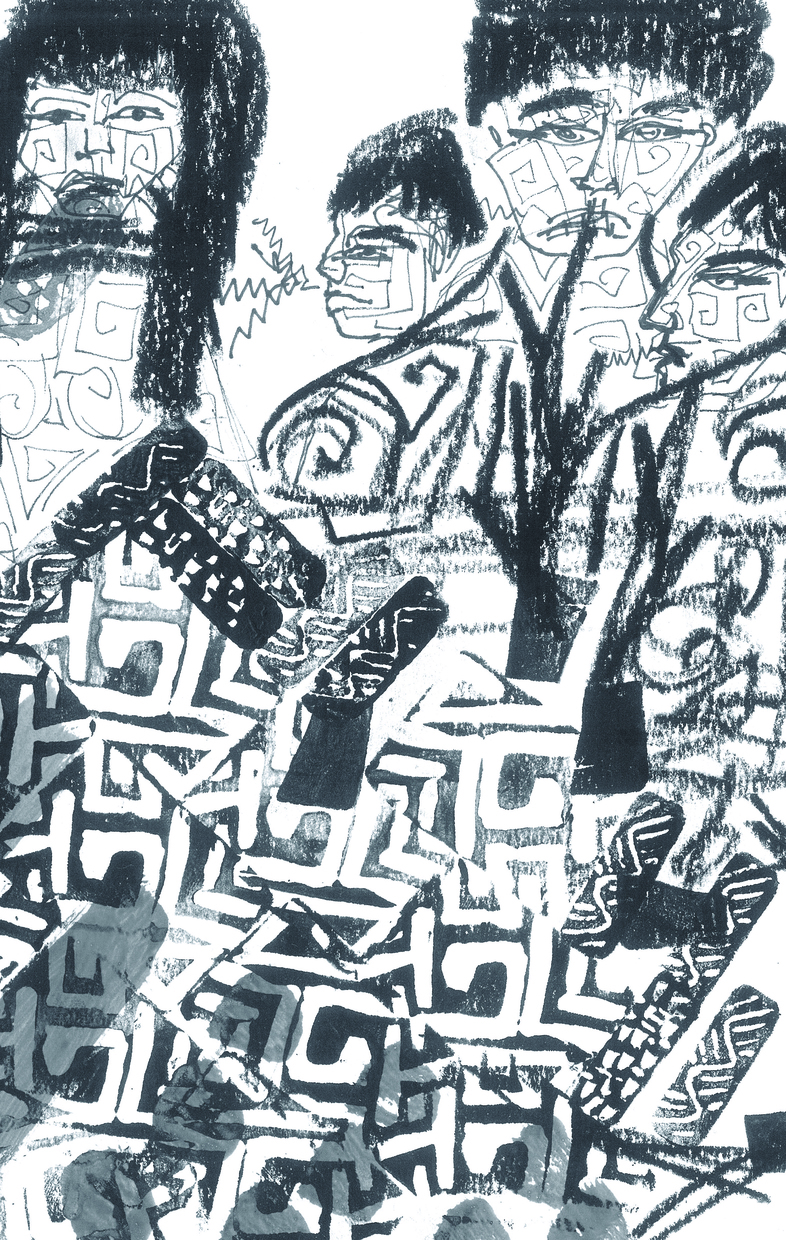
\includegraphics[width=152mm]{./imgs/img6.pdf}
\end{figure}

\chapter*{}

\mbox{}\vspace*{\fill}

% \begin{verse}
% Não podendo mais comer milho verde,\\
% a velha chorou e quis virar tatu.\\
% Foi sozinha para o mato e cavou um buraco.
% \end{verse}

% \begin{verse}
% \textit{Yuxabu haska waa, ana hawa pitima,\\
% kaxaaya. Yuxabu yaixi ka katsi eskani kiaki.\\
% Ha mesti ni medan kaxun, kini waaya.}
% \end{verse}

\letra{N}{ão} podendo mais comer milho verde,
a velha chorou e quis virar tatu.
Foi sozinha para o mato e cavou um buraco.

\vspace{2em}

\letra{Y}{uxabu} haska waa, ana hawa pitima,
kaxaaya. Yuxabu yaixi ka katsi eskani kiaki.
Ha mesti ni medan kaxun, kini waaya.

\vspace*{\fill}

\pagebreak
\thispagestyle{empty}
\begin{figure}
\vspace*{-.5cm}
\hspace*{-2.2cm}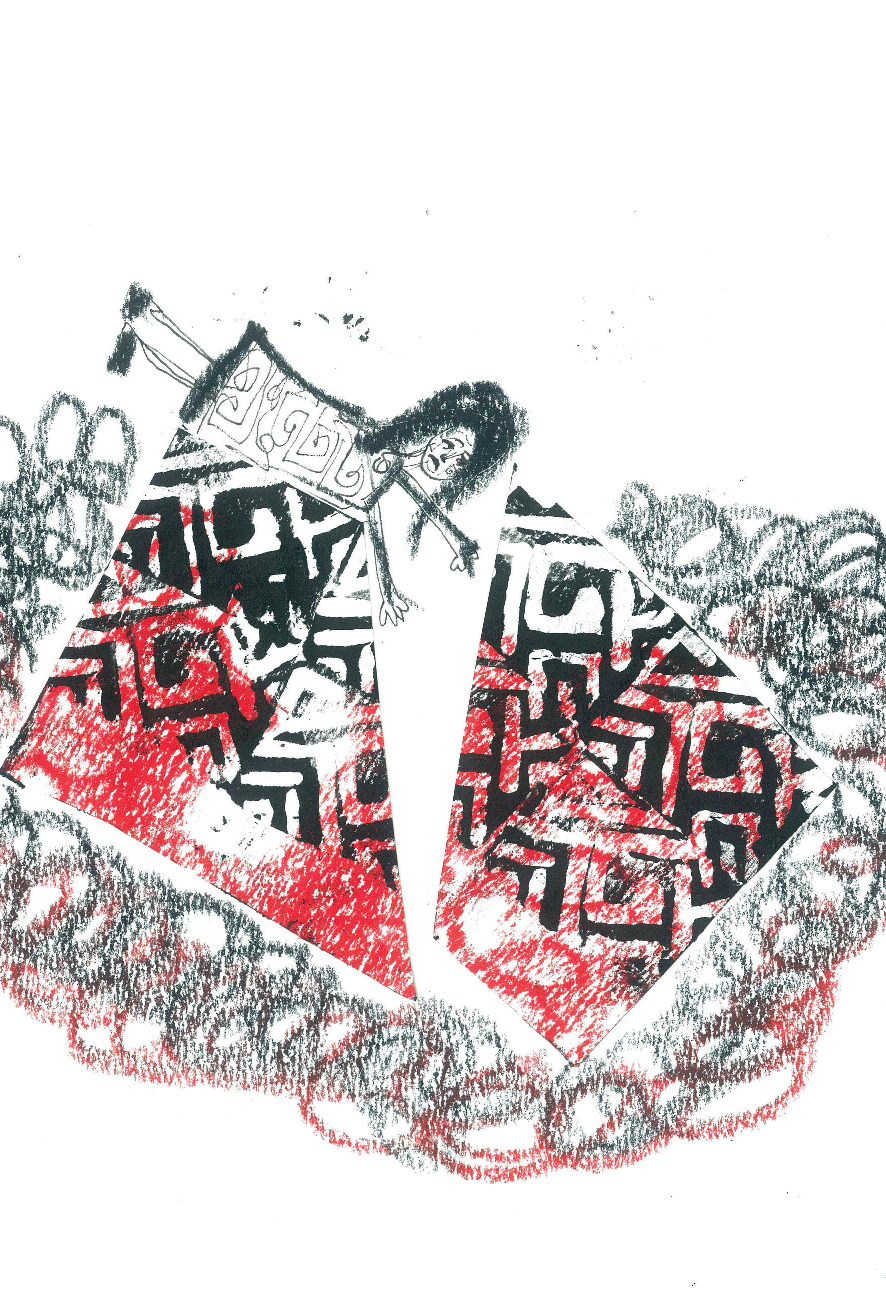
\includegraphics[width=138mm]{./imgs/img7.pdf}
\end{figure}

\chapter*{}

\mbox{}\vspace*{\fill}

% \begin{verse}
% Um homem que havia ido caçar a viu\\
% cavando o buraco, aproximou-se\\
% dela e lhe perguntou:\\
% --- Ei, velha, por que você\\
% está cavando um buraco?\\
% --- É porque não posso comer milho seco.\\
% Só posso comer milho verde. Mas como\\
% esculhambaram comigo, vim cavar um\\
% buraco para ser tatu, respondeu.\\
% O homem a escutou e ficou pensativo,\\
% chorando tristemente.
% \end{verse}

% \begin{verse}
% \textit{Huni piaya kaxun, yuxabun kini\\
% waa, betxia, hunin yuxabu yukaa:\\
% --- Yuxabun, min hawa\\
% katsi kini waai? aka.\\
% --- En haska waxun, piti kuxi\\
% pitima, xeki patxi besti en piaya,\\
% ea itxabu, huxun, en kini waai\\
% yaix katsidan, aka.\\
% Hunin ninkaa, hawen\\
% dabanen iki, kaxaaya.}
% \end{verse}

\letra{U}{m} homem que havia ido caçar a viu
cavando o buraco, aproximou-se
dela e lhe perguntou:\break
--- Ei, velha, por que você
está cavando um buraco?\break
--- É porque não posso comer milho seco.
Só posso comer milho verde. Mas como
esculhambaram comigo, vim cavar um
buraco para ser tatu, respondeu.\break
O homem a escutou e ficou pensativo,
chorando tristemente.

\vspace{2em}

\letra{H}{uni} piaya kaxun, yuxabun kini
waa, betxia, hunin yuxabu yukaa:\break
--- Yuxabun, min hawa
katsi kini waai? aka.\break
--- En haska waxun, piti kuxi
pitima, xeki patxi besti en piaya,
ea itxabu, huxun, en kini waai
yaix katsidan, aka.\break
Hunin ninkaa, hawen
dabanen iki, kaxaaya.

\vspace*{\fill}

\pagebreak
\thispagestyle{empty}
\begin{figure}
\vspace*{-2cm}
\hspace*{-2.8cm}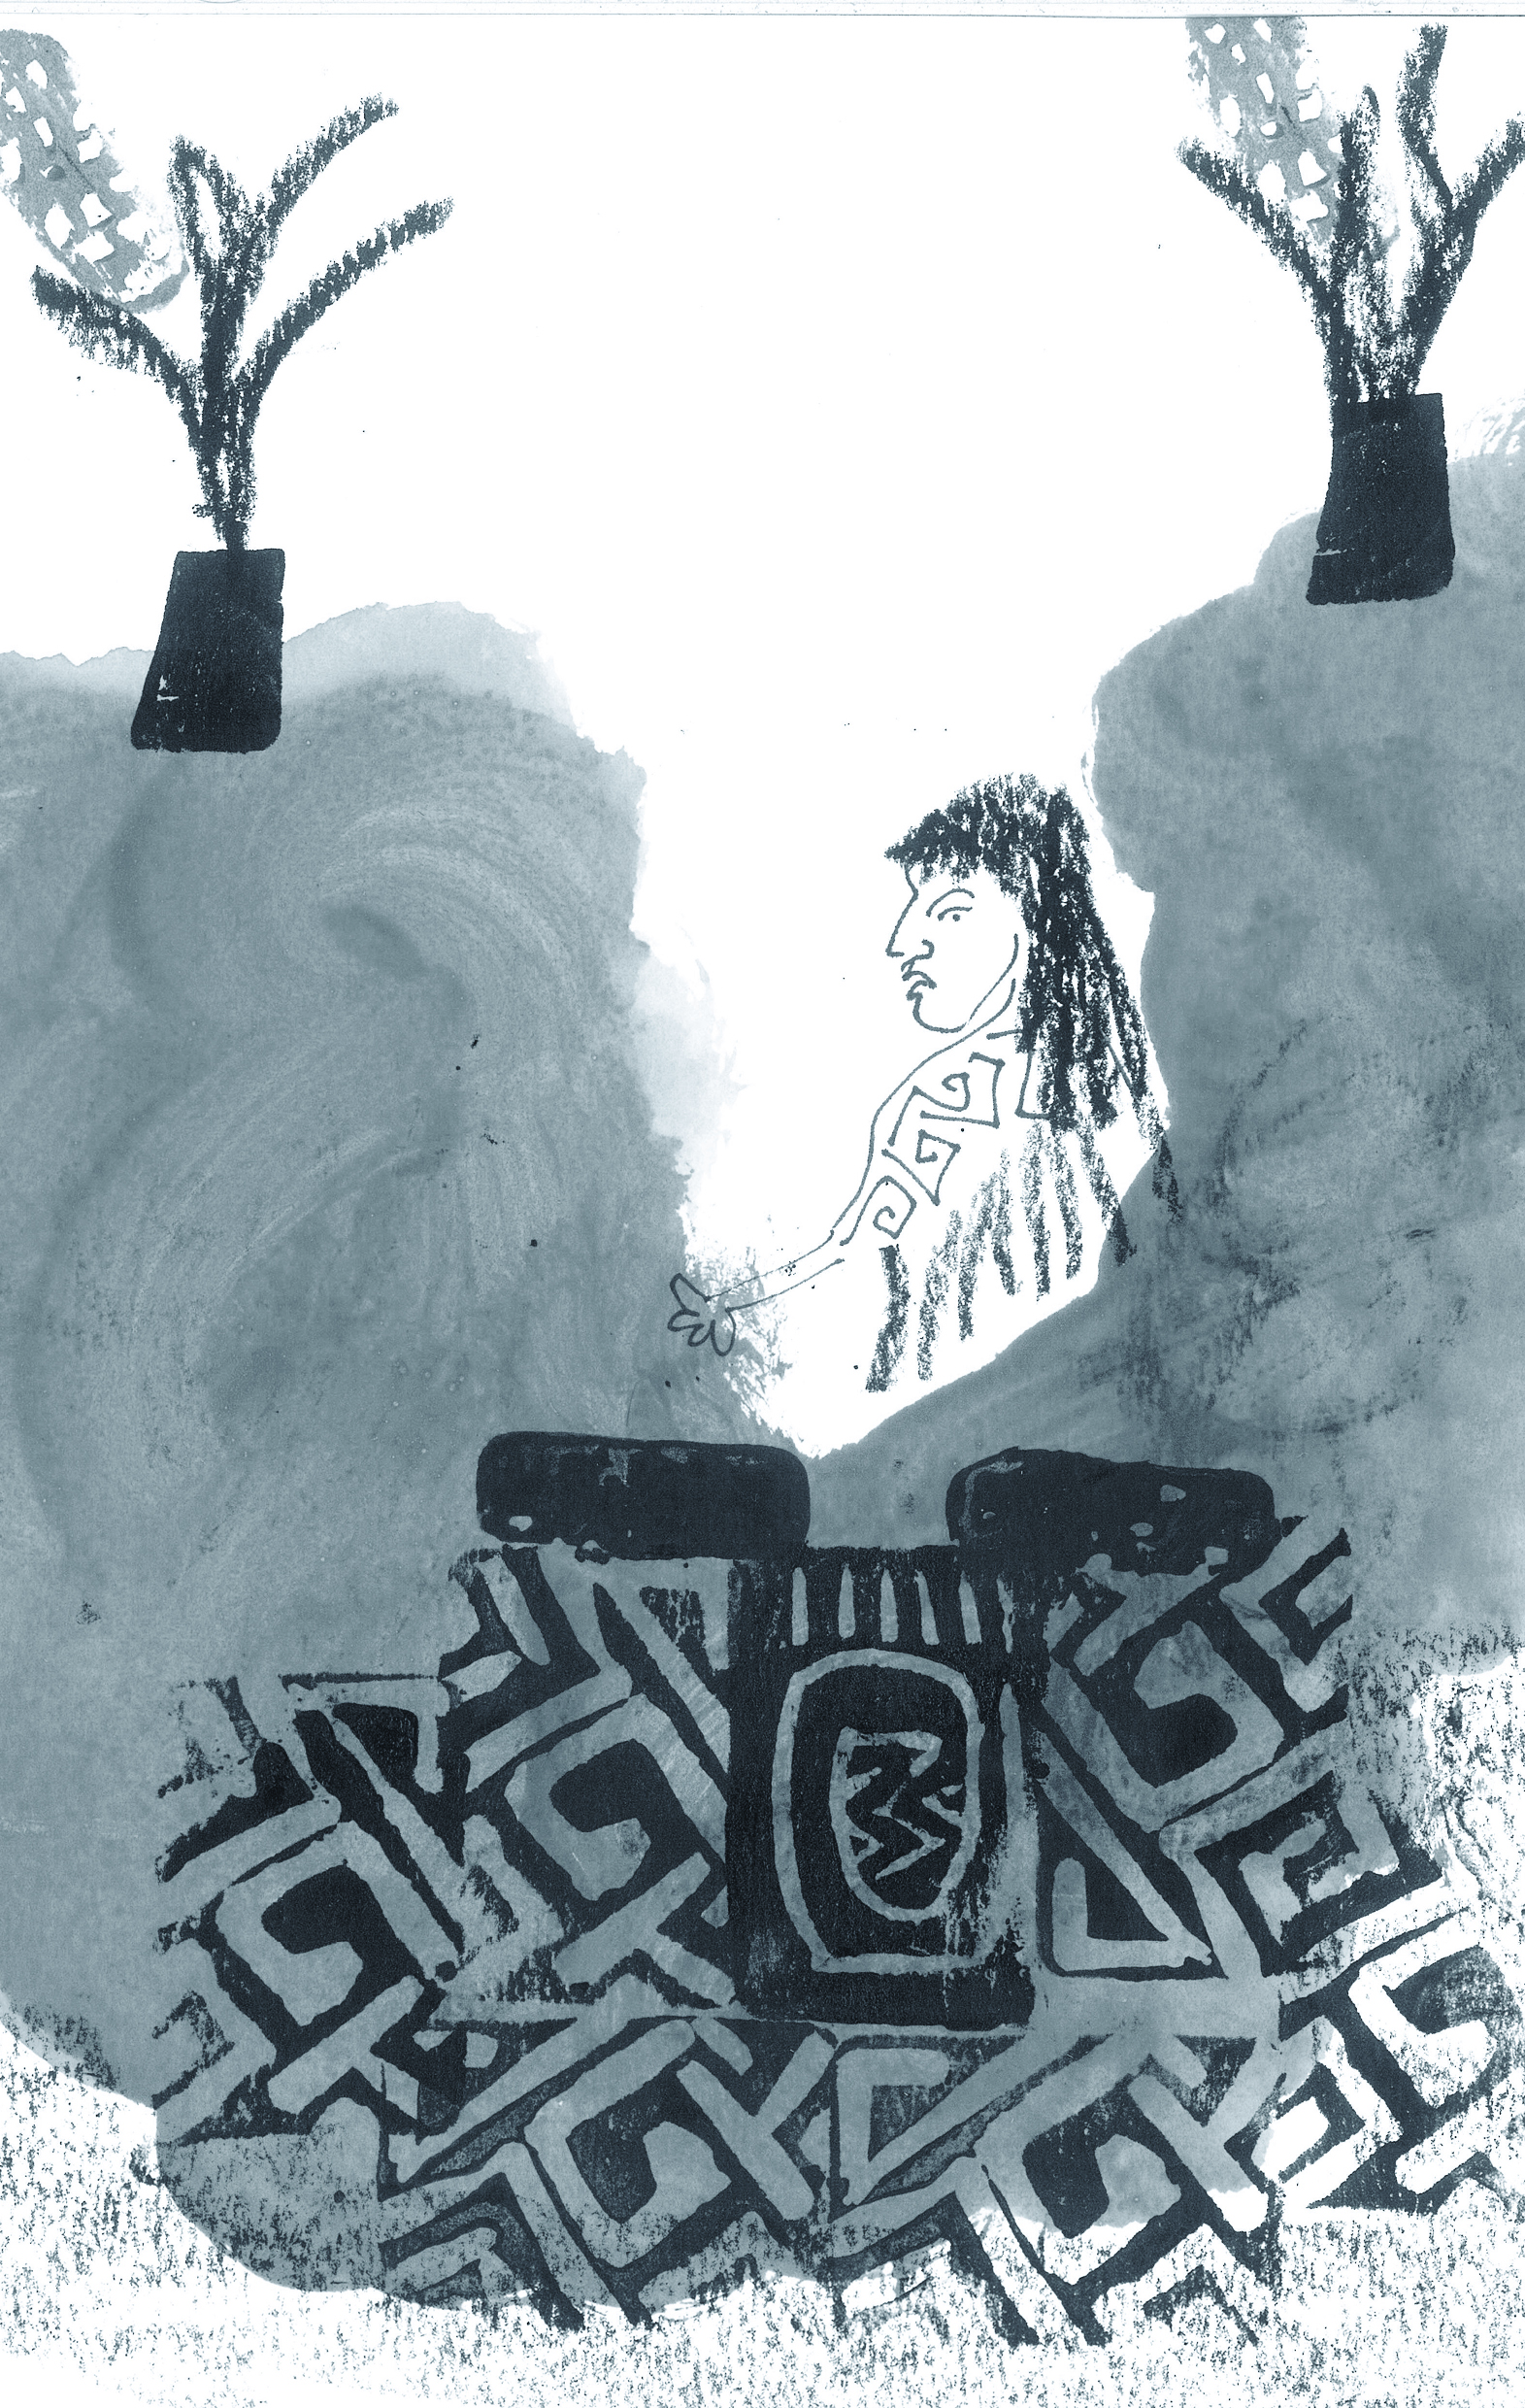
\includegraphics[width=150mm]{./imgs/img8.pdf}
\end{figure}

\chapter*{}

\mbox{}\vspace*{\fill}

% \begin{verse}
% Ao regressar, pergunto\\
% à família dela:\\
% --- Por que vocês\\
% esculhambaram com a velha?\\
% --- Esculhambei porque ela só\\
% comia o milho verde do meu\\
% roçado. Eu a insultei e\\
% ela foi embora.\\
% --- A velha foi para lá cavar\\
% buraco, eu a vi. Ela quer virar\\
% tatu — disse o caçador.
% \end{verse}

% \begin{verse}
% \textit{Haska wabidani, hukidan,\\
% hawen nabu yuia:\\
% --- En nabun, mi hawa\\
% katsi yuxabu\\
% itxa kamen, aka.\\
% --- Habia en xeki patxi\\
% ea pianaya,\\
% en itxaa, kaaki, aka.\\
% --- Yuxabudan uani kini\\
% waai, en uinbidanxuki,\\
% yaix katsidan, aka.}
% \end{verse}

\letra{A}{o} regressar, pergunto
à família dela:\break
--- Por que vocês
esculhambaram com a velha?\break
--- Esculhambei porque ela só
comia o milho verde do meu
roçado. Eu a insultei e
ela foi embora.\break
--- A velha foi para lá cavar
buraco, eu a vi. Ela quer virar
tatu — disse o caçador.

\vspace{2em}

\letra{H}{aska} wabidani, hukidan,
hawen nabu yuia:\break
--- En nabun, mi hawa
katsi yuxabu
itxa kamen, aka.\break
--- Habia en xeki patxi
ea pianaya,
en itxaa, kaaki, aka.\break
--- Yuxabudan uani kini
waai, en uinbidanxuki,
yaix katsidan, aka.

\vspace*{\fill}

\pagebreak
\thispagestyle{empty}
\begin{figure}
\vspace*{-.5cm}
\hspace*{-2.2cm}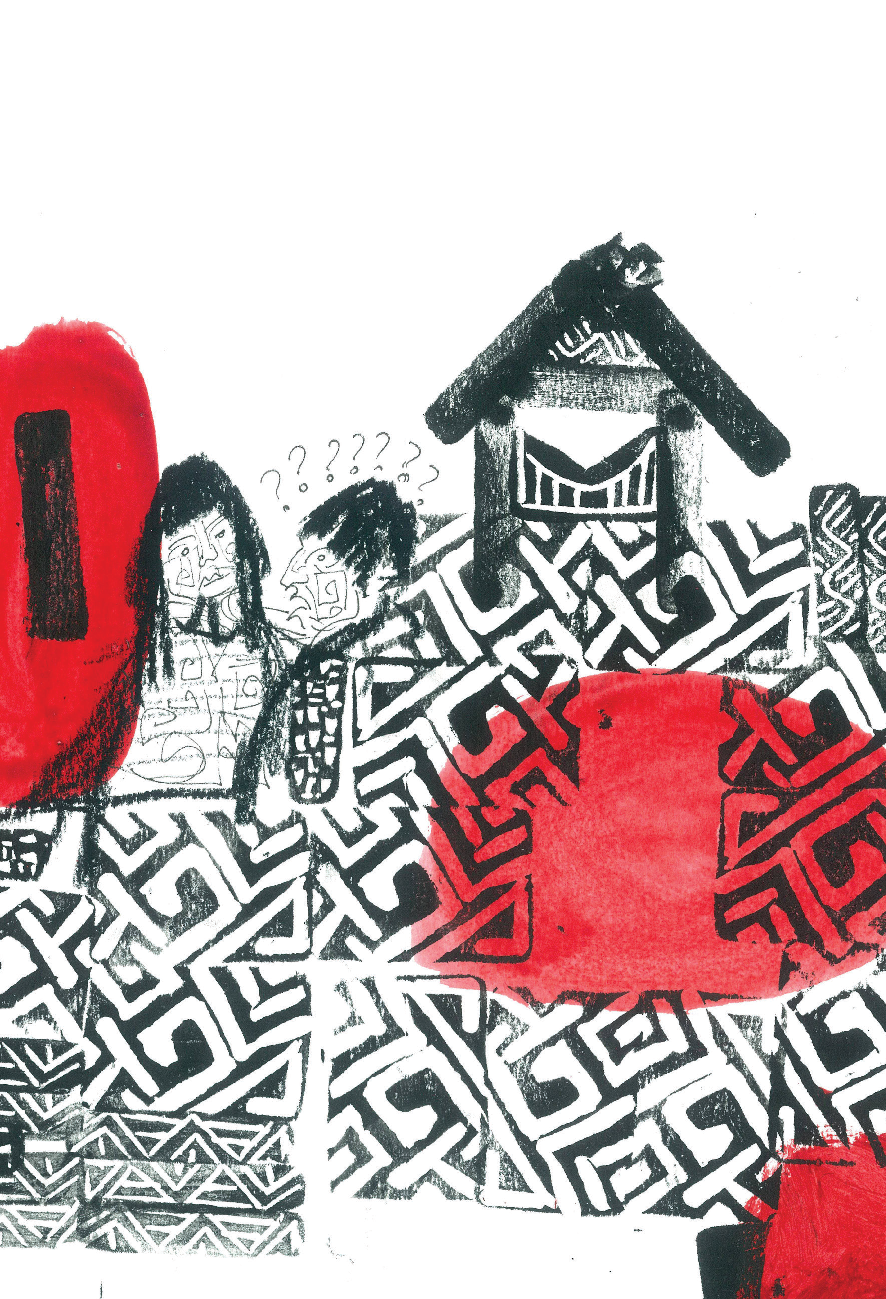
\includegraphics[width=138mm]{./imgs/img9.pdf}
\end{figure}

\chapter*{}

\mbox{}\vspace*{\fill}

% \begin{verse}
% O caçador disse ao seu\\
% filho que estava chorando:\\
% --- A velha que vocês esculhambaram\\
% já virou tatu. Ela já tem rabo, casco\\
% nas costas, casco na cabeça. Virou\\
% todinha tatu. A velha sente falta\\
% do filho. \textit{Vou buscá-lo}, disse a\\
% si mesma. Chamou por ele, gritando\\
% \textit{ruu}, fazendo barulho de tatu.
% \end{verse}

% \begin{verse}
% \textit{Hawen bake yuia, kaxaaya.\\
% --- Yuxabu ma yaixa. Hanunkain, hinayatan,\\
% pexakayatan, nuxakayatan, buxakayatan.\\
% Haska wakin, keyua. Yuxabu hawen bake\\
% manui: \emph{En bake itannun} ika. \emph{Huu} aka.}
% \end{verse}

\letra{O}{caçador} disse ao seu
filho que estava chorando:\break
--- A velha que vocês esculhambaram
já virou tatu. Ela já tem rabo, casco
nas costas, casco na cabeça. Virou
todinha tatu. A velha sente falta
do filho.\break 
\textit{Vou buscá-lo}, disse a
si mesma. Chamou por ele, gritando
\textit{ruu}, fazendo barulho de tatu.

\vspace{2em}

\letra{H}{awen} bake yuia, kaxaaya.\break
--- Yuxabu ma yaixa. Hanunkain, hinayatan,
pexakayatan, nuxakayatan, buxakayatan.\break
Haska wakin, keyua. Yuxabu hawen bake
manui:\break 
\emph{En bake itannun} ika. \emph{Huu} aka.

\vspace*{\fill}

\pagebreak
\thispagestyle{empty}
\begin{figure}
\vspace*{-1cm}
\hspace*{-2.2cm}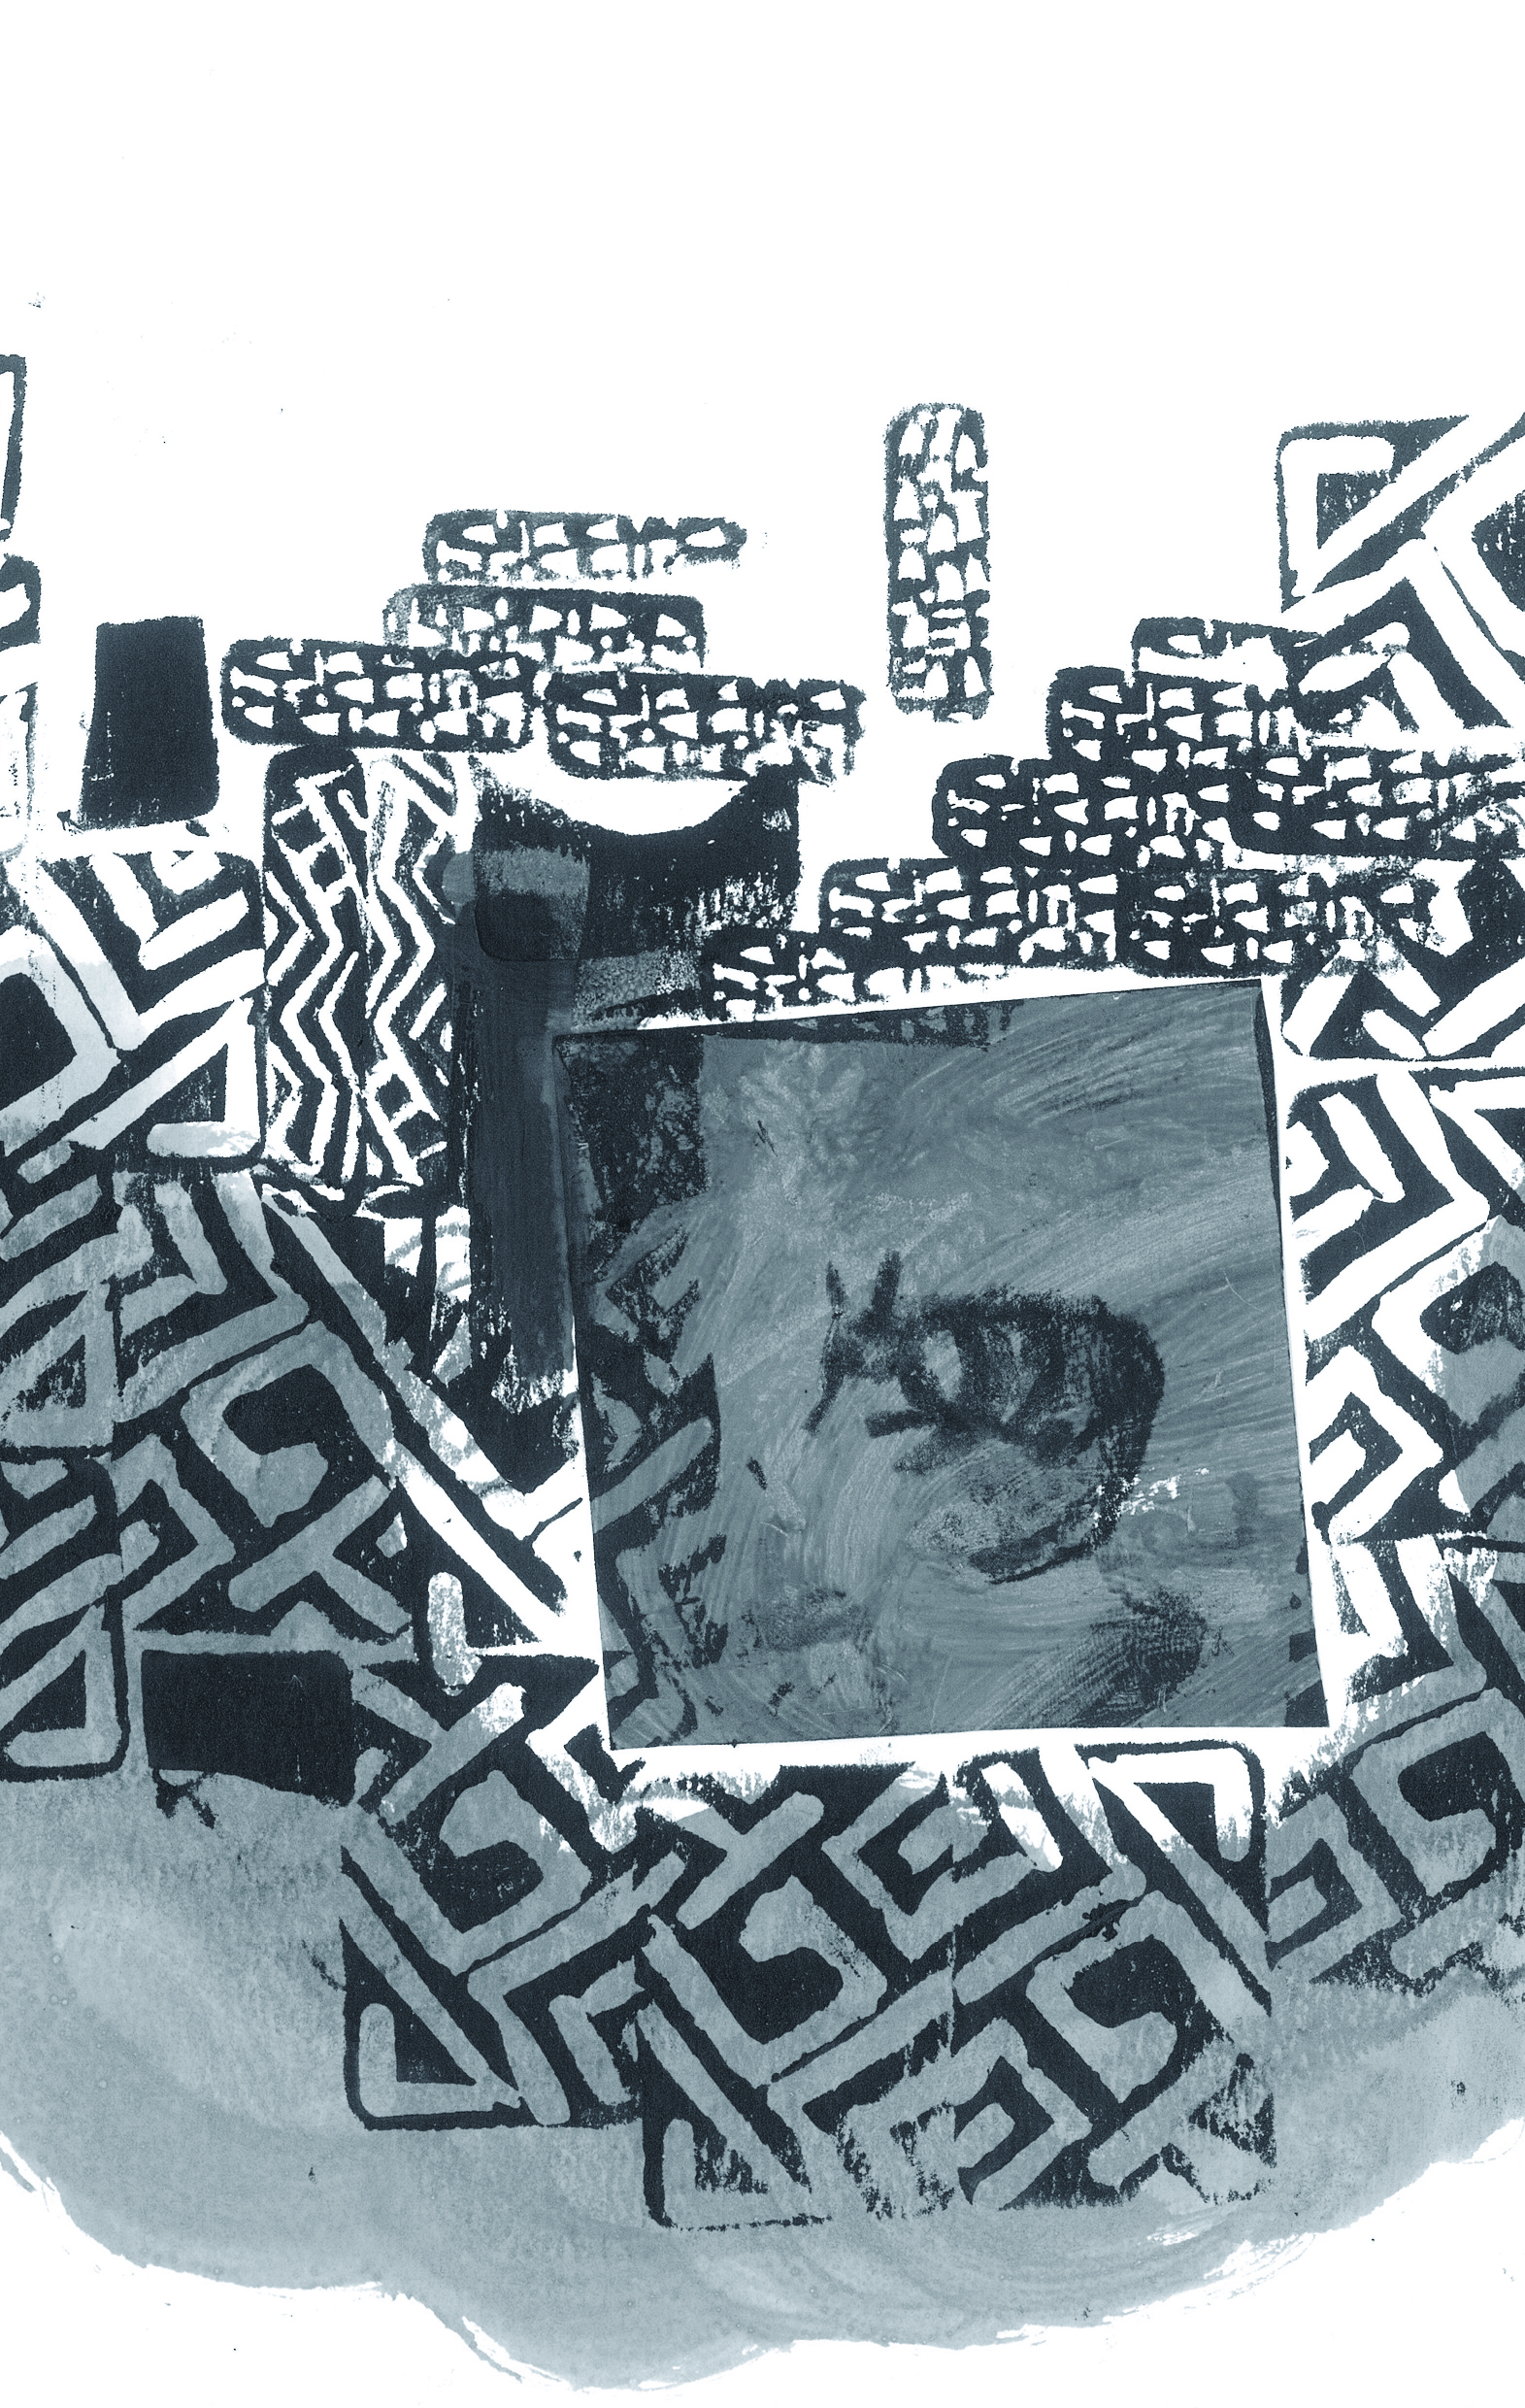
\includegraphics[width=138mm]{./imgs/img10.pdf}
\end{figure}

\chapter*{}

\mbox{}\vspace*{\fill}

% \begin{verse}
% O seu filho pequeno sentia falta\\
% da mãe, e chorava sem parar.\\
% Ele andava sozinho, chorando,\\
% de um lado para o outro.\\
% A velha ouviu o choro e pensou:\\
% --- O meu filho está chorando, vou vê-lo.\\
% Voltou à aldeia para vê-lo; lá estava ele\\
% sentado, chorando. Quando viu o tatu,\\
% alegrou-se, e o tatu lhe disse:\\
% --- Meu filho, eu vou te levar.
% \end{verse}

% \begin{verse}
% \textit{Hawen bake hawen ibu\\
% manui, kaxawankainkainaya.\\
% Hawen bake, ha mesti bai\\
% tanai, kaxakukuaya.\\
% Yuxabu kaxai ninkaa:\\
% --- En bake kaxaai, uintannun, ika.\\
% Huaya, bake pixta kaxai, tsauken,\\
% bake pixta yaix betxia, benimaaya.\\
% Yaixin bake pixta yuikin:\\
% --- En bake, en mia yuai, aka.}
% \end{verse}

\letra{O}{seu} filho pequeno sentia falta
da mãe, e chorava sem parar.
Ele andava sozinho, chorando,
de um lado para o outro.
A velha ouviu o choro e pensou:\break
--- O meu filho está chorando, vou vê-lo.
Voltou à aldeia para vê-lo; lá estava ele
sentado, chorando. Quando viu o tatu,
alegrou-se, e o tatu lhe disse:\break
--- Meu filho, eu vou te levar.

\vspace{2em}

\letra{H}{awen} bake hawen ibu
manui, kaxawankainkainaya.
Hawen bake, ha mesti bai
tanai, kaxakukuaya.
Yuxabu kaxai ninkaa:\break
--- En bake kaxaai, uintannun, ika.
Huaya, bake pixta kaxai, tsauken,
bake pixta yaix betxia, benimaaya.
Yaixin bake pixta yuikin:\break
--- En bake, en mia yuai, aka.

\vspace*{\fill}

\pagebreak
\thispagestyle{empty}
\begin{figure}
\vspace*{-.5cm}
\hspace*{-2.2cm}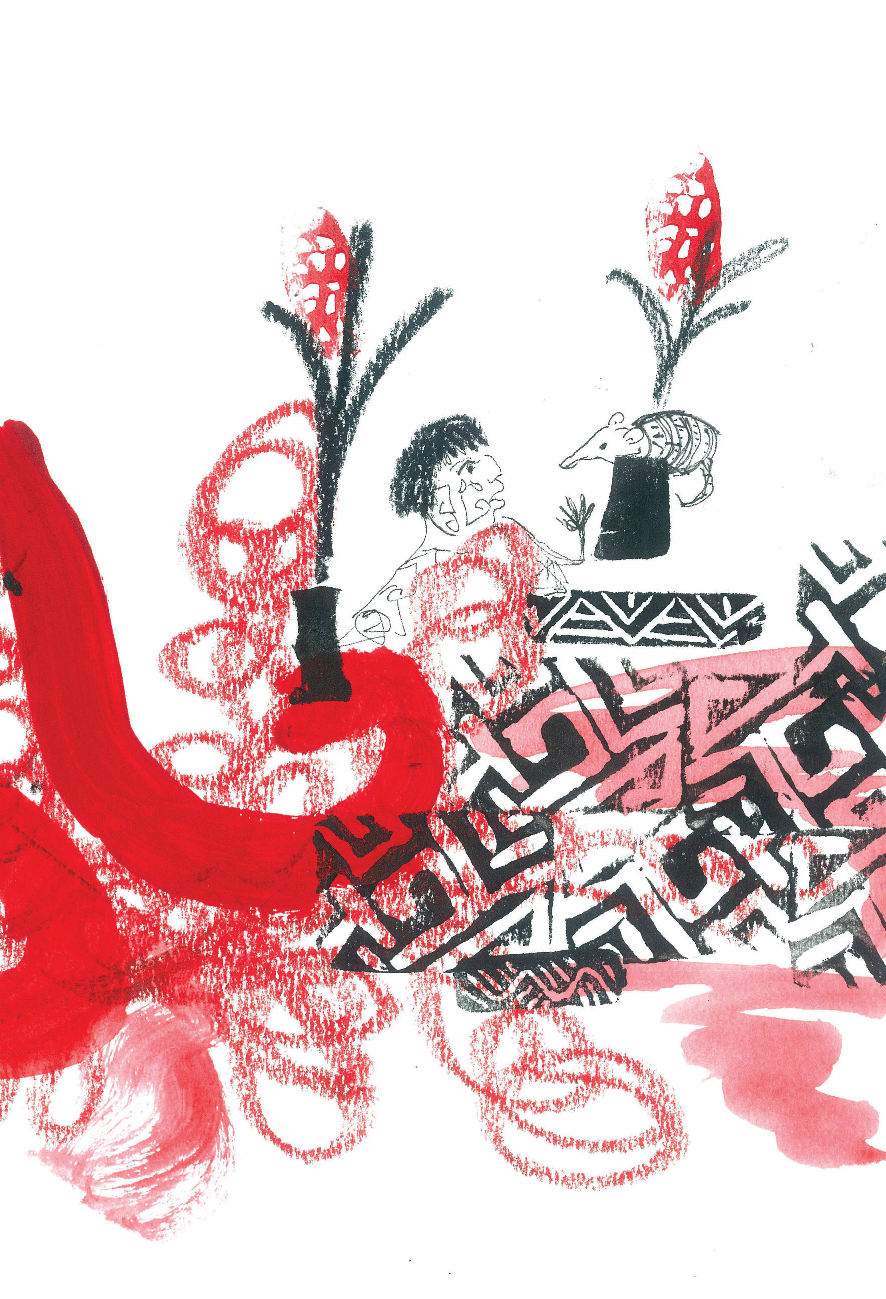
\includegraphics[width=138mm]{./imgs/img11.pdf}
\end{figure}

\chapter*{}

\mbox{}\vspace*{\fill}

% \begin{verse}
% A criança que estava\\
% sentada ficou contente.\\
% Então a velha levou o menino\\
% para morar dentro do buraco.\\
% Ela lhe fez o rabo, o casco das\\
% costas, o casco da cabeça.\\
% E a criança ficou feliz.\\
% A velha havia feito a mesma\\
% coisa para virar tatu.
% \end{verse}

% \begin{verse}
% \textit{Bake pixta benimaai, tsauken.\\
% Hanunkain, yuxabun bake pixta\\
% hawen hiwe medan yukin.\\
% Bake pixta hina waxun, pexaka\\
% waxun, buxaka waxun.\\
% Haska waxun, bake pixta\\
% benimani kiaki.\\
% Yuxabudan eskani kiaki,\\
% yaix katsidan.}
% \end{verse}

\letra{A}{criança} que estava
sentada ficou contente.
Então a velha levou o menino
para morar dentro do buraco.
Ela lhe fez o rabo, o casco das
costas, o casco da cabeça.
E a criança ficou feliz.
A velha havia feito a mesma
coisa para virar tatu.

\vspace{2em}

\letra{B}{ake} pixta benimaai, tsauken.
Hanunkain, yuxabun bake pixta
hawen hiwe medan yukin.
Bake pixta hina waxun, pexaka
waxun, buxaka waxun.
Haska waxun, bake pixta
benimani kiaki.
Yuxabudan eskani kiaki,
yaix katsidan.

\vspace*{\fill}

\pagebreak
\thispagestyle{empty}
\begin{figure}
\vspace*{-2cm}
\hspace*{-2.8cm}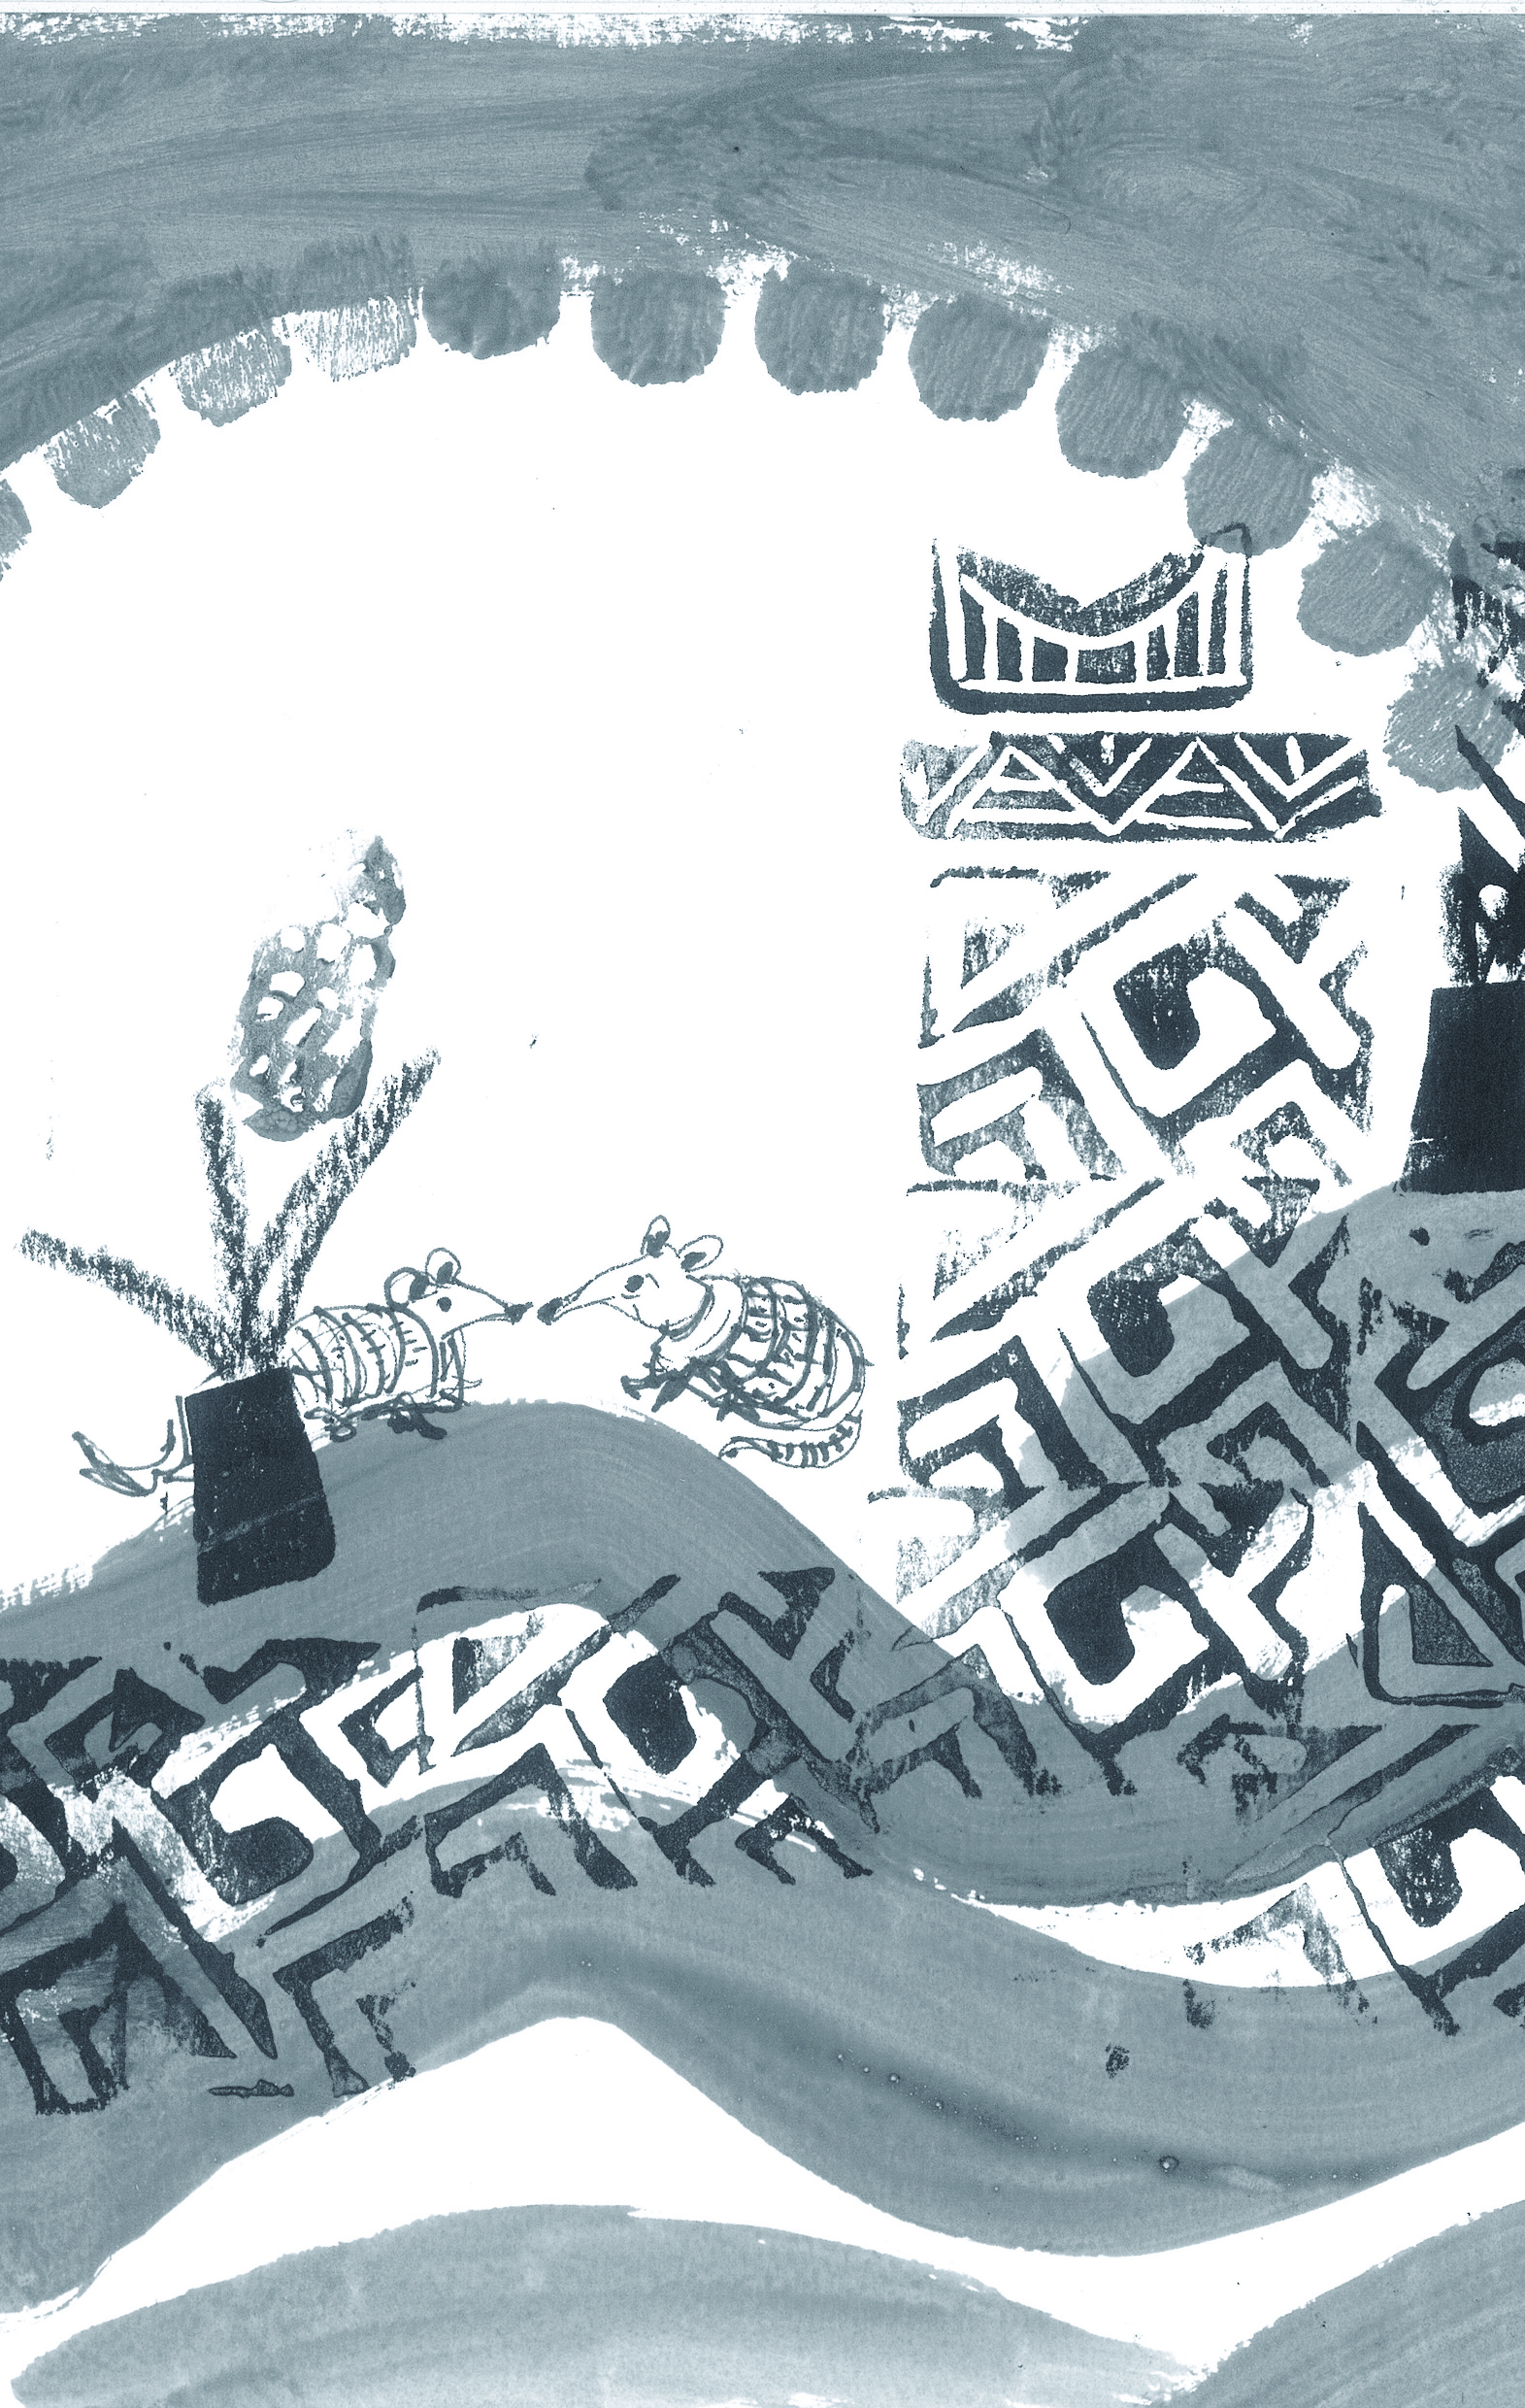
\includegraphics[width=150mm]{./imgs/img12.pdf}
\end{figure}

\chapter*{}

\mbox{}\vspace*{\fill}

% \begin{verse}
% A história diz que quem\\
% domesticou a batata doce para\\
% podermos comer foi o tatu, e\\
% quando não tinha batata doce\\
% para comer, o tatu comia minhoca.\\
% Foi assim que a velha fez para\\
% virar tatu, transformou o corpo\\
% e passou a comer batata doce e,\\
% quando não tinha, comia minhoca.
% \end{verse}

% \begin{verse}
% \textit{Kadi bikindan, yaixin bini kiaki.\\
% Kadimakendan yaixdan\\
% xena besti pimis kiaki.\\
% Yuxabudan eskani kiaki, yaix\\
% katsidan. Hatixunki, yamaki}
% \end{verse}

\letra{A}{história} diz que quem
domesticou a batata doce para
podermos comer foi o tatu, e
quando não tinha batata doce
para comer, o tatu comia minhoca.
Foi assim que a velha fez para
virar tatu, transformou o corpo
e passou a comer batata doce e,
quando não tinha, comia minhoca.

\vspace{2em}

\letra{K}{adi} bikindan, yaixin bini kiaki.
Kadimakendan yaixdan
xena besti pimis kiaki.
Yuxabudan eskani kiaki, yaix
katsidan. Hatixunki, yamaki.

\vspace*{\fill}

\pagebreak
\thispagestyle{empty}
\begin{figure}[H]
\vspace*{-.5cm}
\hspace*{-2.2cm}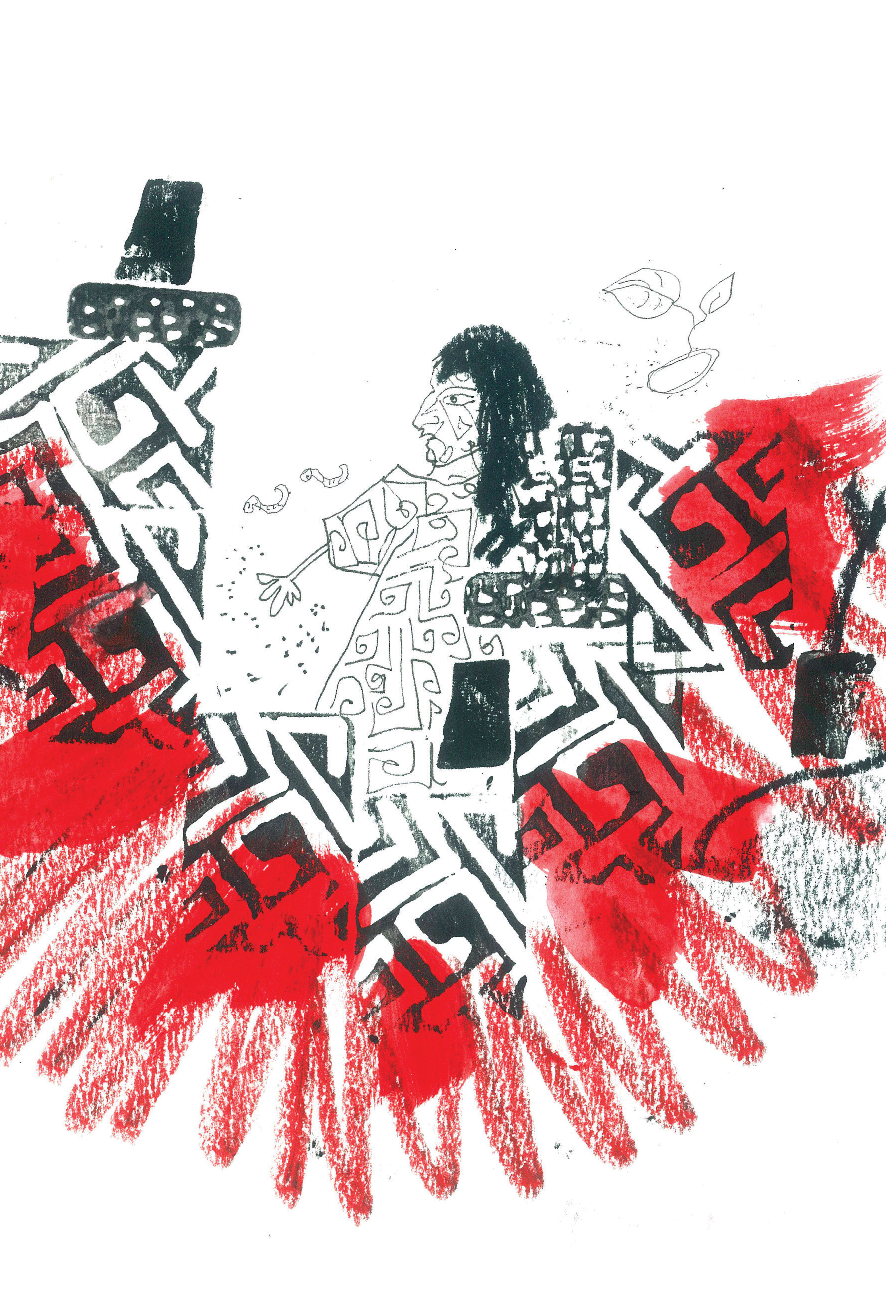
\includegraphics[width=138mm]{./imgs/img13.pdf}
\end{figure}

\endgroup



